% 图 70.3 —— **结构化重画**（2026-09-25，替换掉 `checks/emit_hand.py` 的逐段拟合稿）
%%
% 结构：一个圆 + 一条过心直径 + 圆周上 4 个实心点 + 7 个文字标签（**无箭头**）
%%
% 旧版是**描摹**：把每一段笔画单独拟合后发出来，连「箭头头」都被当成"一条很粗的短线"描
%   （图 81.5 上一度出现 `\draw[line width=7.0pt] (586,277)--(586,270);` 这种 7px 长的疙瘩），
%   渲染出来是黑疙瘩而不是箭头。本版改成**看懂结构后用 TikZ 画**。
%%
% 做法、约定、已踩过的坑 → `＜工作区＞\checks\redraw\README_重画流程.md`
% 本图圆/椭圆的中心与半径、标签的文字与位置，沿用 probe 的脚手架（那部分它是对的）。
%%
% ⚠ 本图 tikzpicture 是 y=-1pt（**y 翻转**）⇒ `arc` 的角向"递减"才是屏幕逆时针；
%   同一根线上的多段弧必须同向。改完务必拿原书并排、放大核箭头朝向。
%%
\documentclass[12pt]{standalone}
\usepackage{fontspec}
\setsansfont{Arial}
\newfontfamily\mfallback{DejaVu Sans}
\usepackage{tikz}
\usetikzlibrary{arrows.meta}
\begin{document}
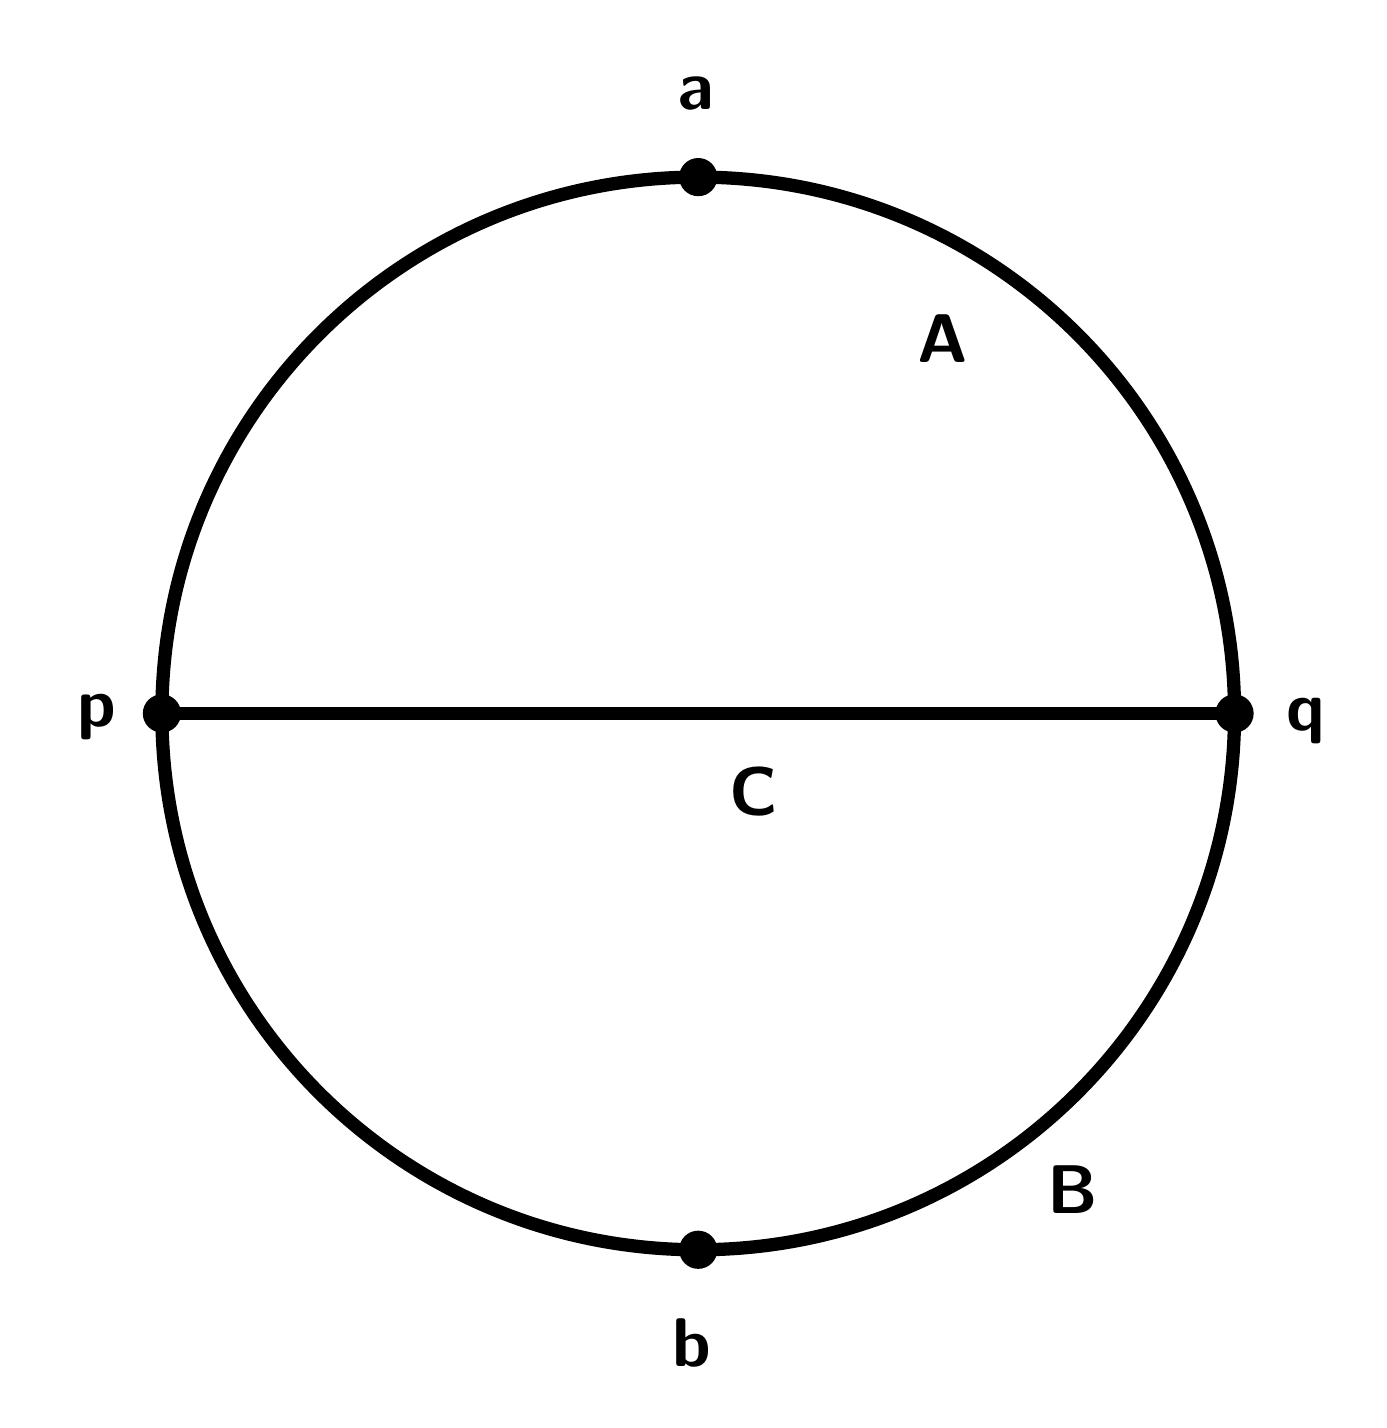
\begin{tikzpicture}[x=1pt, y=-1pt, line width=4.8pt, line cap=round, line join=round]

  % ── 圆：中心 (242.3,247.8)、半径 193.8（prims2 的 ellipses）──
  \draw (242.3,247.8) circle (193.8);

  % ── 直径 pq：两端恰为圆上左右两点 ──
  \draw (48.5,247.8) -- (436.1,247.8);

  % ── 圆周上的 4 个实心点：上 a / 下 b / 左 p / 右 q ──
  \foreach \x/\y in {242.3/54.0, 242.3/441.6, 48.5/247.8, 436.1/247.8}
    \fill (\x,\y) circle (6.9);

  % ── 7 个标签（\x/\y/字号/字母）──
  %    坐标＝原书实测的**墨迹盒中心**，再按首轮渲染实测的「盒心 vs 字形墨心」偏差回修过
  \foreach \x/\y/\sz/\lab in {%
      241.78/24.02/33.7/a,
      330.58/112.27/29.8/A,
      24.82/249.11/30.7/p,
      461.72/250.63/30.7/q,
      262.45/276.18/32.2/C,
      377.48/419.77/31.5/B,
      240.02/475.16/31.3/b}
    \node[anchor=center,inner sep=0pt,font=\fontsize{\sz}{42.1}\selectfont] at (\x,\y) {\textsf{\textbf{\textit{\lab}}}};

  % 钉死画布（W/H 取自 prims2）
  \path[use as bounding box] (0,0) rectangle (481,496);
\end{tikzpicture}
\end{document}
